\section{Theoretical Analysis}
\label{sec:analysis}

In order to make our theoretical analysis we made use of two well-known methods, Mesh Method and  Nodal Method, since its use allow us to make a system of equations that determine our theoretical values.

\subsection{Mesh Method}

By using the Mesh Method we introduce currents that circulate in the meshes of the circuit as shown in Figure~\ref{fig:Circuit_Mesh}, and then evaluate the circuit based on the new currents.

\begin{figure}[h] \centering
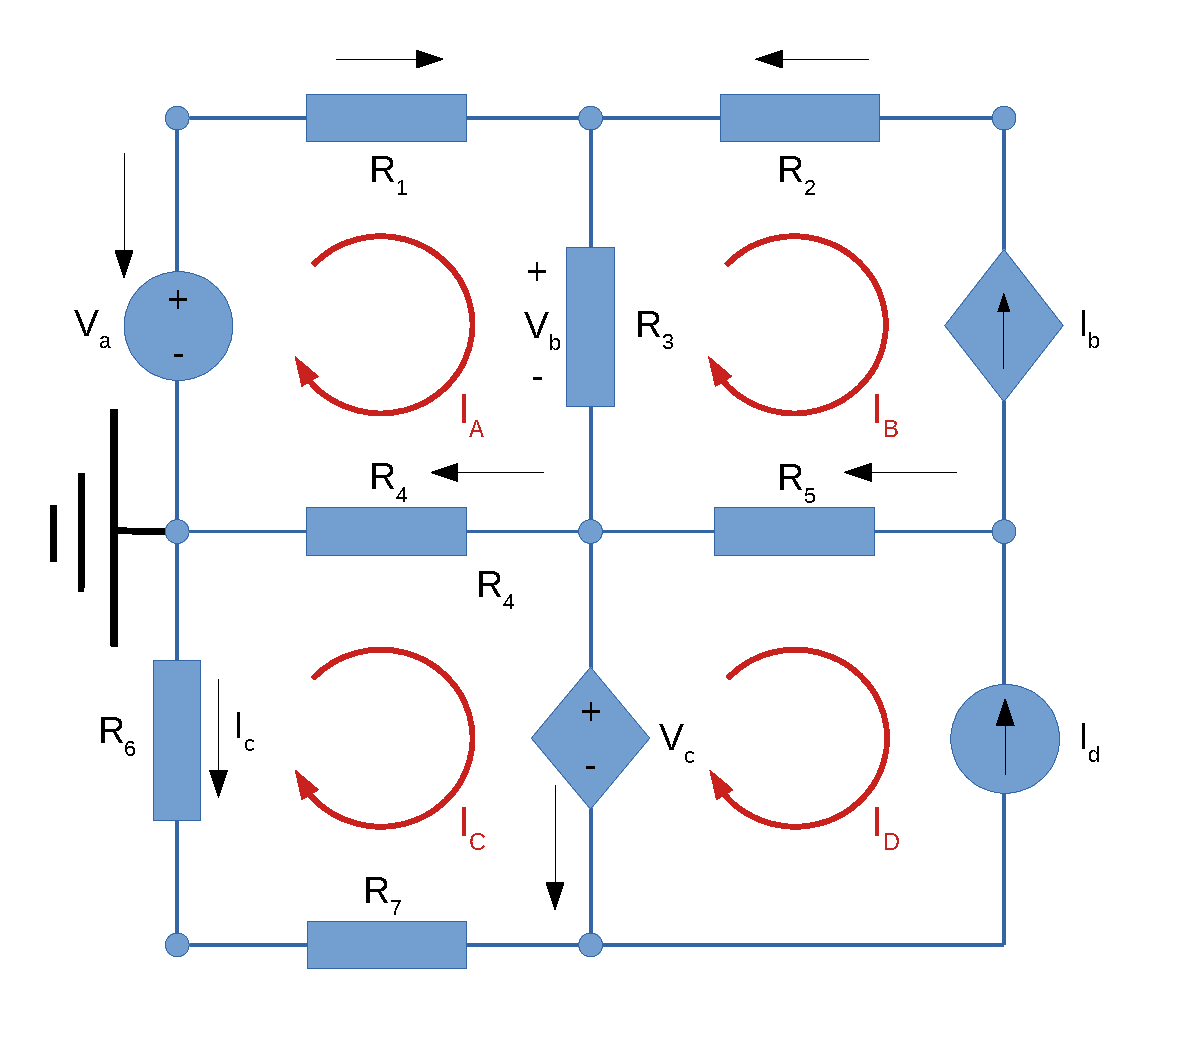
\includegraphics[width=0.5\linewidth]{CircuitMesh.pdf}
\caption{Circuit analysed with mesh currents.}
\label{fig:Circuit_Mesh}
\end{figure}

After identifying the mesh currents, we used the Kirchhoff Voltage Law~(KVL) in the left meshes (Mesh~$\alpha$~ and Mesh~$\delta$~).

\begin{equation}
 V_a= R_1I_a + V_{\beta} + R_4(I_{\alpha} - I_{\delta});
  \label{eq:MM_Alpha}
\end{equation}
\begin{equation}
  R_6I_{\delta} + R_4(I_{\delta} + V_{\delta} + R_7I_{\delta} = 0;
  \label{eq:MM_Delta}
\end{equation}

Besides that we know that I_b=I_{\beta} , I_d=-I_{\gamma} and I_c=-I_{\delta}.

At this point we have 5 equations with 8 unknown variables (I_{\alpha}, I_{\beta}, I_{\delta}, I_b, I_c, I_d, V_{\beta}, V_{\delta}).
It is required more 3 equations that add more information in order to get the same number of unkonwn variables and equations. 
\begin{equation}
 V_{\delta}=K_{\delta}I_{\delta}
  \label{eq:Vc}
\end{equation}
\begin{equation}
  I_{\beta}=K_{\beta}V_{\beta}
  \label{eq:Ib}
\end{equation}
\begin{equation}
V_{\beta}=R_3(I_a-I_b)
\end{equation}


The solution to this linear system of equations is determined by Octave:

\begin{table}[h]
  \centering
  \begin{tabular}{|l|r|}
    \hline    
    {\bf Variables} & {\bf Value [A or V]} \\ \hline
    I_{A} & 1.067284e-03 \\ \hline 
I_{B} & 1.118444e-03 \\ \hline 
I_{C} & 0.000000e+00 \\ \hline 
I_{D} & -1.019408e-03 \\ \hline 
@V_{b} & -1.541489e-01 \\ \hline 
@V_{c} & -0.000000e+00 \\ \hline 
I_{b} & -1.118444e-03 \\ \hline 
I_{c} & -0.000000e+00 \\ \hline 

  \end{tabular}
  \caption{Variables in the Mesh Method. A variable preceded by @ is of type {\em current} and expressed in Ampere; other variables are of type {\em voltage} and expressed in Volt.}
  \label{tab:malhas}
\end{table}

\subsection{Nodal Method}

In this subsection we make use of the other method (Nodal Method) to determinate the values of current and voltage by finding first all the knots in the circuit, as made in Figure~\ref{fig:Circuit_Nodal}.

\begin{figure}[H] 
\centering
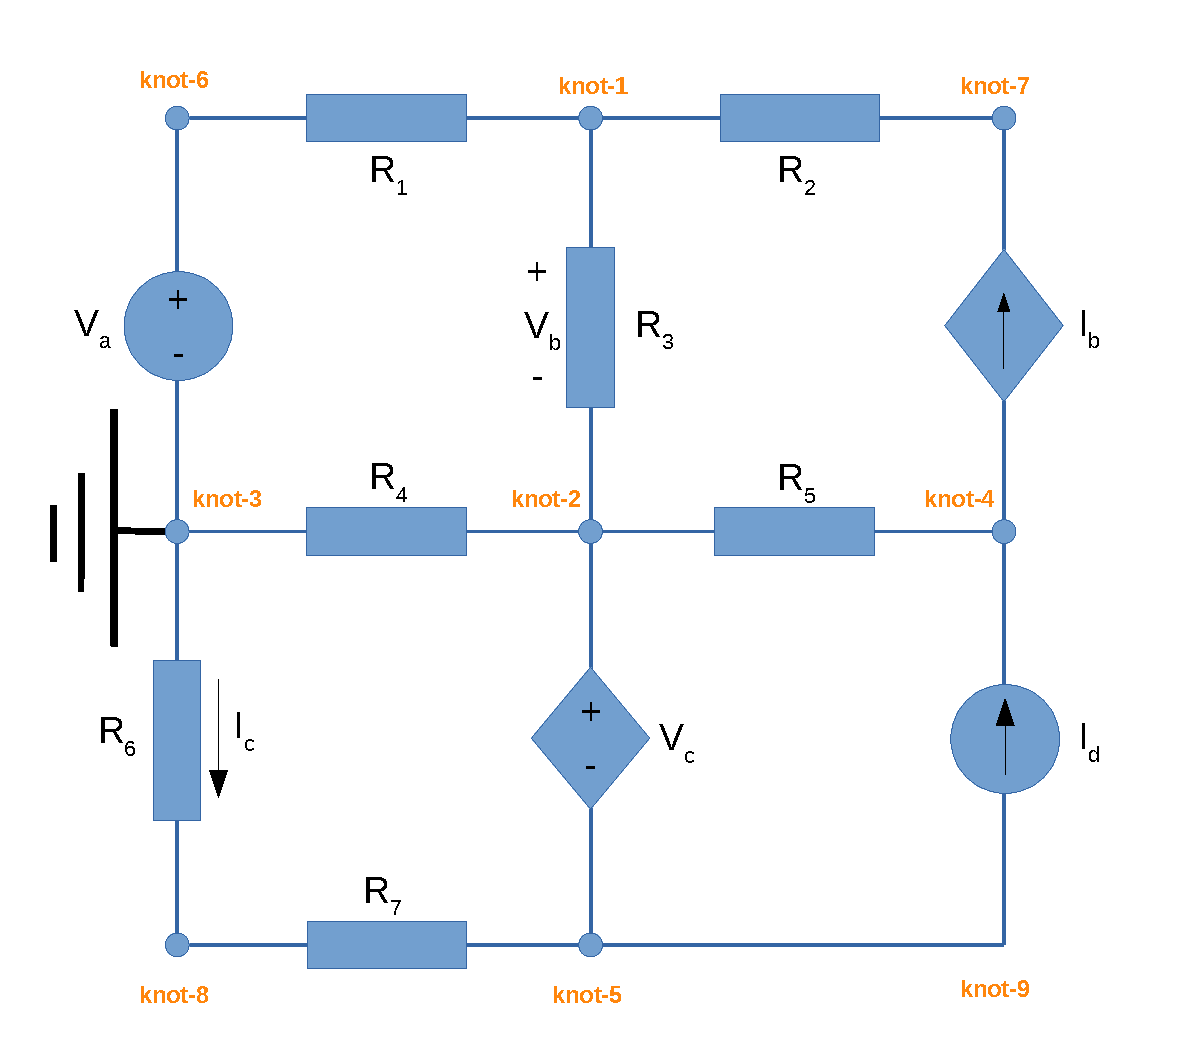
\includegraphics[width=0.5\linewidth]{CircuitNodal.pdf}
\caption{Circuit analysed with nodal voltages.}
\label{fig:Circuit_Nodal}
\end{figure}

After finding all the knots we apply KCL (Kirchhoff Current Law) to all the knots except knots 2, 3, 5 and 6 because they are connected to tension sources.
Note that v_i is a reference to the potencial in knot i.

\begin{equation}
  \frac{v_6-v_1}{R_1} + \frac{v_7-v_1}{R_2} = \frac{V_b}{R_3};
\end{equation}
\begin{equation}
  I_{\beta} = \frac{v_7-v_1}{R_2};	
\end{equation}
\begin{equation}
  I_{\gamma} = \frac{v_4-v_2}{R_5}+I_{\beta};
\end{equation}
\begin{equation}
  I_{\delta} = \frac{v_8-v_5}{R_7};
\end{equation}

We also know that:

\begin{equation}
  V_{\alpha}= v_6-v_3;
\end{equation}
\begin{equation}
  V_{\beta}= v_1-v_2.
\end{equation}
\begin{equation}
  V_{\delta}= v_2-v_5.
\end{equation}

And we have the same equations determinated using Meshes Method:
\begin{equation}
 V_{\beta}=K_{\beta}I_{\beta}
\end{equation}
\begin{equation}
 V_{\delta}=K_{\delta}I_{\delta}
\end{equation}

Using Ohm’s Law, we find the relation:
\begin{equation}
  I_c = \frac{v_3-v_8}{R_6}.
  \label{eq:NM_OhmIc}
\end{equation}

At this point we have 10 equations and 12 unkown variables, so we need 2 more equations that add the information that we need to determinate our final linear system of equations.
We can establish v_2=0 and by continuity of the current in the tension sources we have: 

\begin{equation}
  I_c + \frac{v_6-v_1}{R_1}= \frac{v_2-v_3}{R_4}.
\end{equation}
The solution to this linear system of equations is determined by Octave:

\begin{table}[h]
  \centering
  \begin{tabular}{|l|r|}
    \hline    
    {\bf Name} & {\bf Value [A or V]} \\ \hline
    V_{1} & 3.878423e-05  \\ \hline 
V_{2} & 1.110223e-16  \\ \hline 
V_{3} & -2.255973e-13  \\ \hline 
V_{4} & 1.890796e+01  \\ \hline 
V_{5} & 7.105387e-01  \\ \hline 
V_{6} & 5.230611e+00  \\ \hline 
V_{7} & -1.074709e+01  \\ \hline 
V_{8} & 6.239231e-01  \\ \hline 
V_{b} & 3.878423e-05  \\ \hline 
V_{c} & -7.105387e-01  \\ \hline 
I_{b} & -5.155393e-03  \\ \hline 
I_{c} & -8.618601e-05  \\ \hline 

  \end{tabular}
  \caption{Variables in the Nodal Method. A variable preceded by @ is of type {\em current} and expressed in Ampere; other variables are of type {\em voltage} and expressed in Volt.}
  \label{tab:nos}
\end{table}

